% Persian Introduction Section
% 
% This section introduces the MultiModal RAG project and the chosen medical textbook

\section{مقدمه}
با رشد روزافزون حجم اطلاعات پزشکی و انتشار مستندات تخصصی در قالب‌های مختلف، دسترسی سریع و دقیق به دانش مورد نیاز در این حوزه به چالشی اساسی تبدیل شده است. کتاب‌های پزشکی تخصصی معمولاً شامل محتوای پیچیده و چندوجهی هستند که ترکیبی از متن، جداول، نمودارها و تصاویر تشخیصی را در بر می‌گیرند. استخراج و بازیابی اطلاعات از این منابع به روش‌های سنتی زمان‌بر و غیرکارآمد است.

در این پروژه، یک سامانه بازیابی اطلاعات چندوجهی مبتنی بر هوش مصنوعی توسعه یافته است که قادر به پردازش هوشمند اسناد پزشکی غیرساختاریافته و ایجاد پایگاه دانش جامع برای پاسخگویی به پرسش‌های تخصصی است. این سامانه از تکنیک‌های پیشرفته پردازش زبان طبیعی، بینایی ماشین و بازیابی تقویت‌شده با تولید \lr{(Retrieval-Augmented Generation - RAG)} بهره می‌برد.

\subsection{منبع داده}
برای ارزیابی و آزمایش سامانه، کتاب \lr{Oxford Textbook of Medicine, 6th Edition} به عنوان منبع اصلی داده انتخاب شده است. این کتاب یکی از معتبرترین و جامع‌ترین مراجع پزشکی در سطح جهان است که توسط انتشارات دانشگاه آکسفورد منتشر شده و شامل چهار جلد و سی بخش تخصصی می‌باشد.

\begin{figure}[h]
    \centering
    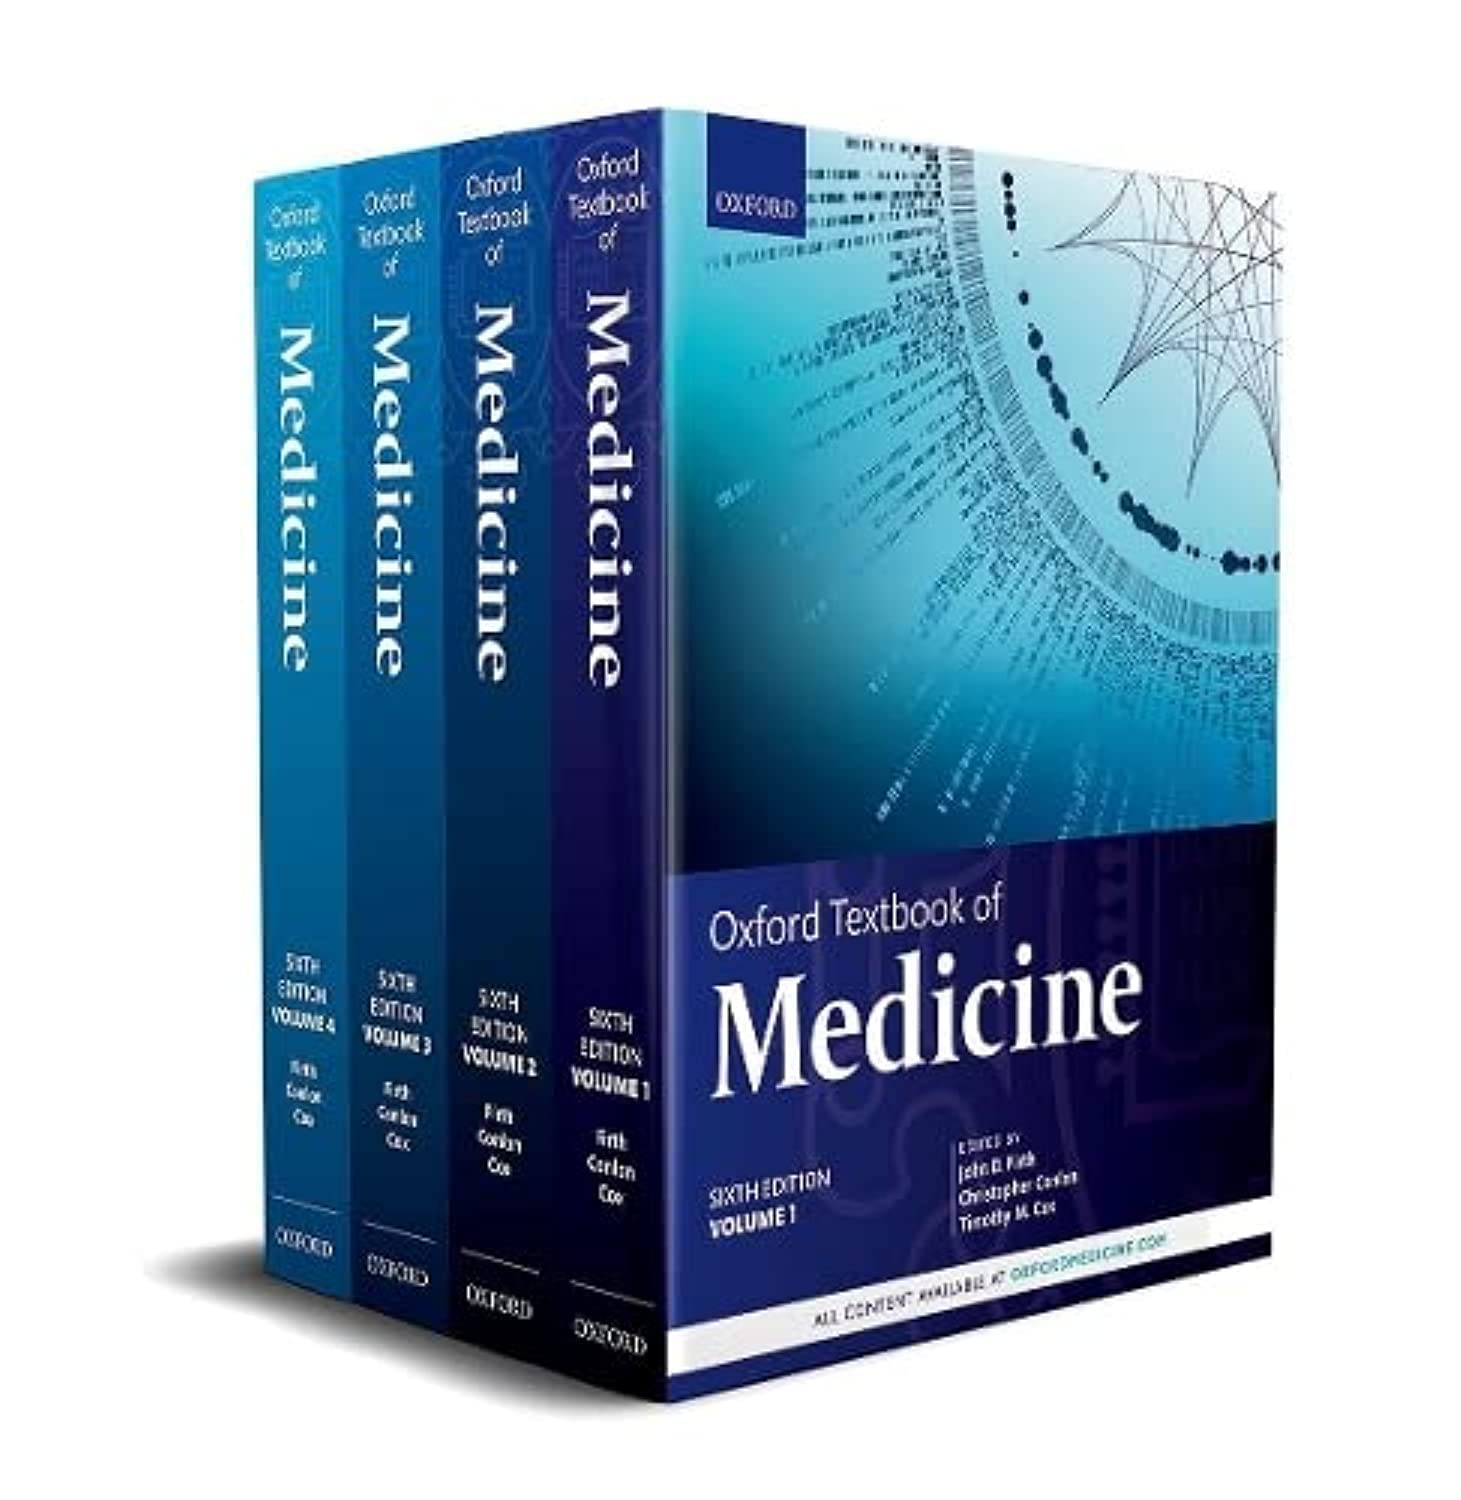
\includegraphics[width=0.5\textwidth]{oxford_cover.jpg}
    \caption{جلد کتاب \lr{Oxford Textbook of Medicine, 6th Edition}}
    \label{fig:oxford_cover}
\end{figure}

\noindent
در این پروژه، جلد دوم این مجموعه که شامل بخش‌های ۱۰ تا ۱۵ است، مورد پردازش قرار گرفته است. این جلد حاوی ۱۸۷۳ صفحه غیرساختاریافته از محتوای پزشکی تخصصی است که طیف وسیعی از موضوعات را پوشش می‌دهد.

\subsection{ویژگی‌های محتوای منبع}
محتوای این جلد دارای ویژگی‌های زیر است که پردازش آن را به چالشی فنی تبدیل می‌کند:

\begin{itemize}
    \item \textbf{ساختار سلسله‌مراتبی پیچیده:} محتوا دارای سطوح متعدد سرفصل، زیربخش و پاراگراف‌های مرتبط است که حفظ این ساختار برای درک صحیح مطالب ضروری است.
    
    \item \textbf{جداول اطلاعاتی متنوع:} صفحات حاوی جداول پیچیده با داده‌های بالینی، آماری و تشخیصی هستند که نیاز به استخراج دقیق و حفظ ساختار دارند.
    
    \item \textbf{محتوای بصری تخصصی:} تصاویر تشخیصی، نمودارها و دیاگرام‌های پزشکی که اطلاعات حیاتی را به صورت بصری منتقل می‌کنند و نیاز به تحلیل هوشمند دارند.
    
    \item \textbf{اصطلاحات تخصصی پزشکی:} استفاده گسترده از واژگان تخصصی، اختصارات و نام‌گذاری‌های علمی که نیاز به پردازش دقیق دارند.
    
    \item \textbf{پیوستگی محتوایی:} ارتباط منطقی بین بخش‌های مختلف که حفظ آن برای درک کامل موضوعات الزامی است.
\end{itemize}

\subsection{اهداف پروژه}
اهداف اصلی این پروژه عبارتند از:

\begin{itemize}
    \item \textbf{تبدیل ساختاریافته:} پردازش اسناد غیرساختاریافته \lr{PDF} و تبدیل آن‌ها به فرمت‌های ساختاریافته با حفظ کامل سلسله‌مراتب و روابط محتوایی.
    
    \item \textbf{پردازش چندوجهی:} استخراج و تحلیل هوشمند متن، جداول و محتوای بصری به صورت یکپارچه.
    
    \item \textbf{نمایه‌سازی هوشمند:} ایجاد پایگاه داده قابل جستجو با حفظ زمینه و ساختار اطلاعات.
    
    \item \textbf{بازیابی دقیق:} پاسخگویی به پرسش‌های تخصصی با استفاده از اطلاعات استخراج‌شده از متن، جداول و تصاویر.
    
    \item \textbf{معماری پاک و قابل توسعه:} طراحی سامانه با رعایت اصول مهندسی نرم‌افزار برای قابلیت نگهداری و توسعه آینده.
\end{itemize}

\subsection{درباره کتاب \lr{Oxford Textbook of Medicine}}
کتاب \lr{Oxford Textbook of Medicine} برجسته‌ترین و معتبرترین کتاب بین‌المللی پزشکی است که به عنوان یک مرجع کلیدی در دفاتر و بخش‌های درمانی پزشکان در سراسر جهان حضور دارد. این کتاب با پوشش بی‌نظیر جنبه‌های علمی و عملکرد بالینی در حوزه طب داخلی و تخصص‌های فرعی آن، همچنین به عنوان منبعی اساسی برای پزشکی قانونی مورد استفاده قرار می‌گیرد.

این اثر جامع، معتبر و بین‌المللی بر ارائه دیدگاه‌های تخصصی و راهنمایی‌های عملی در مدیریت بالینی و پیشگیری از بیماری‌ها تمرکز دارد. بخش‌های مقدماتی این کتاب بر تجربه بیمار، اخلاق پزشکی و تصمیم‌گیری بالینی متمرکز است و فلسفه‌ای انسانی و تفکربرانگیز را ارائه می‌دهد که همواره مشخصه این اثر بوده است. این کتاب به دنبال القای درکی عمیق از نقش پزشکی در جامعه و مشارکت آن در سلامت جمعیت است و از بحث درباره جنبه‌های بحث‌برانگیز پزشکی مدرن طفره نمی‌رود.

\noindent
ویژگی‌های برجسته این کتاب عبارتند از:

\begin{itemize}
    \item \textbf{یکپارچگی علوم پایه و عمل بالینی:} ادغام بی‌نظیر دانش علمی و کاربردهای بالینی در سراسر کتاب، همراه با توضیح پیامدهای تحقیقات برای عملکرد پزشکی.
    
    \item \textbf{پوشش جامع بیماری‌های عفونی:} جامع‌ترین پوشش بیماری‌های عفونی که در هیچ کتاب پزشکی دیگری یافت نمی‌شود.
    
    \item \textbf{موضوعات تخصصی متنوع:} شامل سلول‌های بنیادی و پزشکی بازساختی، نابرابری‌های سلامت، جنبه‌های پزشکی آلودگی و تغییرات اقلیمی، پزشکی سفر و اکسپدیشن، بیوتروریسم و پزشکی قانونی، درد، اختلالات پزشکی در بارداری، تغذیه، و روانپزشکی.
    
    \item \textbf{بخش پزشکی اورژانسی:} طراحی شده برای دسترسی سریع به اطلاعات در مواقع نیاز فوری.
    
    \item \textbf{دسترسی دیجیتال و چاپی:} امکان دسترسی چندگانه بر اساس نیاز و ترجیح کاربران، همراه با به‌روزرسانی‌های منظم در نسخه آنلاین.
    
    \item \textbf{پایگاه مدارک و مراجع پیشرو:} استفاده از جدیدترین یافته‌های تحقیقاتی و شواهد علمی.
\end{itemize}

\noindent
ویرایش ششم این کتاب با بهبودهای قابل توجهی همراه بوده است که در پاسخ به بازخوردهای مستمر کاربران انجام شده است. افزودن بخش‌های خلاصه فصل‌ها برای ارائه دید کلی از محتوا، طراحی جدید برای سهولت خواندن و ناوبری، و همچنین دسترسی رایگان به نسخه آنلاین \lr{Oxford Medicine Online} برای خریداران نسخه چاپی، از جمله این بهبودها هستند.

\noindent
در فصل‌های بعدی، جزئیات معماری سامانه، روش‌های پردازش اسناد، الگوریتم‌های نمایه‌سازی و نتایج ارزیابی به تفصیل ارائه خواهد شد.
